\section{Modularisation}
\label{sec:module}

\subsection{Record/Replay}
Lors de la fonction \textit{update} du moteur, on ajoute la sérialisation des commandes à une Json::Value \textit{jsonval}. Cette Json::Value est enregistrée dans le fichier \textit{replay.txt} lors de l'appel du destructeur du moteur. On enregistre également une seed pour la fonction rand() utilisée dans le jeu.
Afin d'enregister les commandes dans le fichier, on ajoute deux méthodes aux commandes: \textit{Serialize} et \textit{Deserialize}.
\par \textbf{Serialize:} défini et retourne une Json::Value \textit{val}. On ajoute à val tous les attribus nécessaires à la création d'une commande (par exemple, \textit{entityID} pour la plupart des commandes). On ajoute également un champ commun à toutes les commandes: \textit{typeCmd} qui définit le type de la commande sérialisée.
\par \textbf{Deserialize:} à partir d'une Json::Value \textit{in}, on désérialise une commande. On reprend tous les arguments correspondant à la commande pour les mettre dans les champs correspondants. Puis on renvoie la commande ainsi initialisée.

On ajoute une méthode \textit{ReadCommand} au moteur afin de lire toutes les commandes du fichier replay.txt. 

\par \textbf{ReadCommand:} prend une Json::Value \textit{val} en entrée. Décompose val en différentes commandes. On analyse le champ "typeCmd" afin de désérialiser la commande correspondante, les attributs variant d'une commande à l'autre. On enregistre toutes les commandes ainsi re-créées dans le vecteur de commandes du moteur, qui les réalisera à l'aide de sa fonction "update".

\subsection{Répartition sur différents threads}
Afin de préparer la séparation sur plusieurs machines (une se chargeant d'éxecuter le moteur: le serveur, et l'autre gérant le rendu: le client) et d'optimiser l'éxecution du jeu, nous allons séparer notre jeu en deux threads. Alors que le thread principal sera responsable du rendu graphique du jeu, le second se chargera de gérer le rendu.

Afin de ne pas afficher une ressource qui est en cours de modification, nous utilisons un mutex, ce qui permet que les parties critiques du code ne soient pas utilisées en meme temps par plusieurs threads séparés. De plus, La communication entre les threads se fait par le biais de pointeurs vers des booléens et vers l'état du jeu. Lors de la mise en réseau du jeu, la communication se fera par l'intermédiaire de fichiers Json.

\subsection{Répartition sur différentes machines : Lobby}
Afin de jouer à un jeu en réseau, il faut que les joueurs puissent se connecter au serveur, ce qui consiste à faire une liste de clients c\^oté serveur. Dans ce but, plusieurs requettes du client vers le serveur ont été implémentées:
\begin{itemize}
    \item \textbf{Requ\^ete GET}:
    \begin{itemize}
        \item /user/<id> si <id> >= 0 : Renvoie toutes les informations sur l'utilisateur correspondant
        \item /user/<id> si <id> < 0 : Renvoie la liste des utilisateurs connectés au serveur.
    \end{itemize}
    \item \textbf{Requ\^ete POST}: /user/<id> change les informations de l'utilisateur correspondant
    \item \textbf{Requ\^ete PUT}: /user crée un nouvel utilisateur avec les données fournies dans la requete
    \item \textbf{Requ\^ete DELETE}: /user/<id> supprime l'utilisateur correspondant
\end{itemize}

\subsection{Répartition sur différentes machines : Jeu}
    Afin de pouvoir jouer au jeu en réseau, le serveur servira de relais afin de transmettre les commandes effectuées par un joueur à l'autre, afin que les deux joueurs soient synchronisés.
    
    Les nouvelles requetes implémentées sont les suivantes:
    
    \begin{itemize}
        \item \textbf{Requ\^ete GET}:
            \begin{itemize}
                \item /command/<id> : Renvoie au joueur <id> les commandes étant à sa destination
                \item /seed : renvoie la seed du jeu.
            \end{itemize}
        \item \textbf{Requ\^ete PUT}:
            \begin{itemize}
                \item /command/<id> : Ajoute une commande à la liste des commandes effectuées par le joueur <id>
                \item /seed : Envoie la seed générée par le joueur et la renvoie. Si une seed a été précedemment générée par un autre client, renvoie la seed de ce dernier.
            \end{itemize}
        \item \textbf{Requ\^ete DELETE}: /command/<id> supprime les commandes du joueur opposé.
    \end{itemize}


\subsection{Conception logiciel}
Le diagramme des classes pour le serveur est présenté en \autoref{uml:server}

Afin de rendre les communications client/serveur plus intuitives, nous avons choisi de créer une classe qui sera chargée de la communication du client: la classe networkManager (\autoref{uml:networkManager}). La méthode InitConnection permettant de put le nom du client vers le serveur et d'initialiser son ID. On peut mettre dans le destructeur du networkManager l'envoi d'une requete Delete avec son id afin de supprimer le joueur de la liste lors de sa déconnexion.

\begin{landscape}
\begin{figure}[p]
\centering
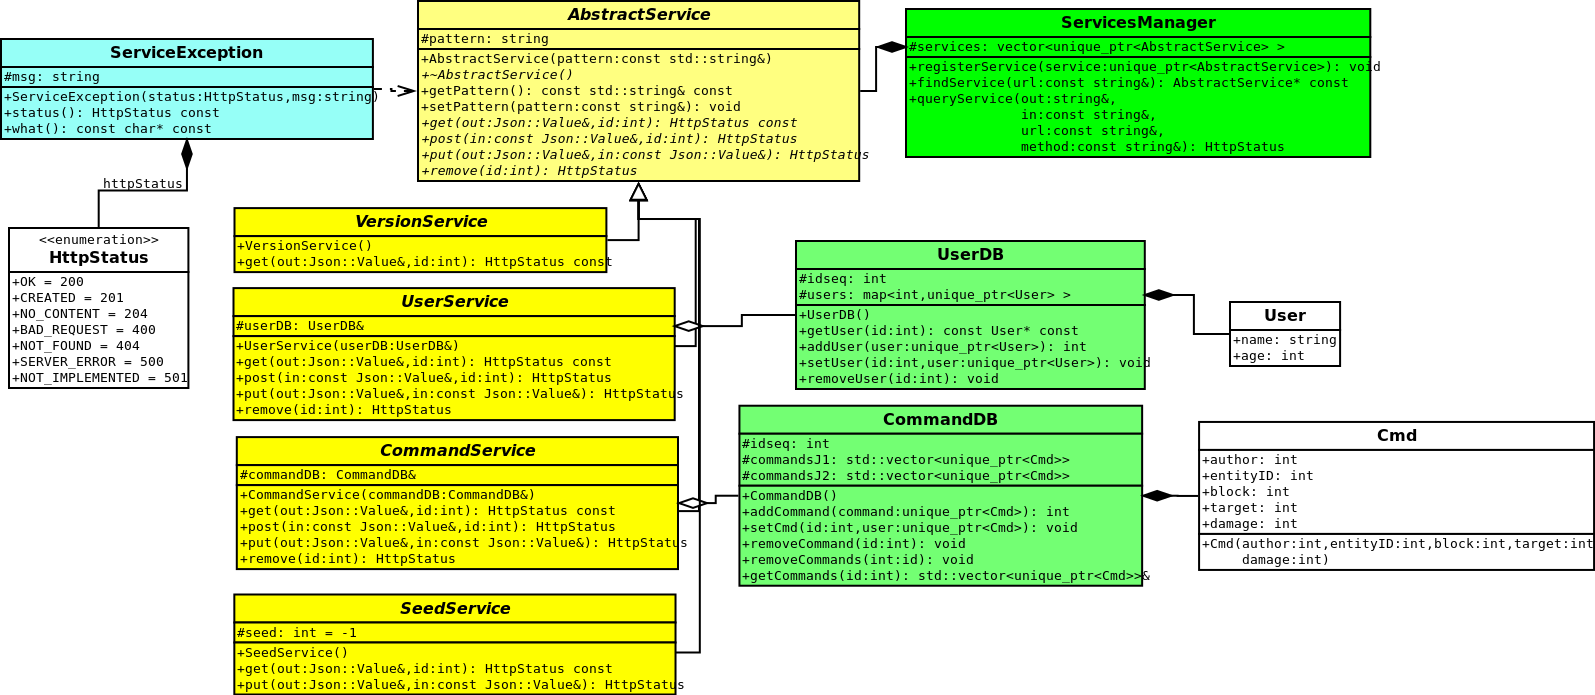
\includegraphics[width=0.9\paperheight]{images/server.png}
\caption{\label{uml:server}Diagramme des classes pour le serveur.} 
\end{figure}
\end{landscape}

\begin{figure}[p]
\centering
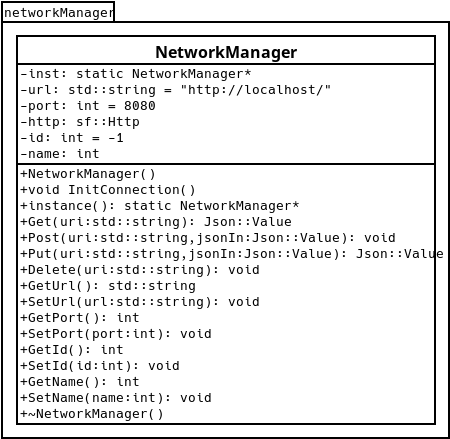
\includegraphics[width=0.4\paperheight]{images/networkManager.png}
\caption{\label{uml:networkManager}Diagramme des classes pour le networkManager.} 
\end{figure}
%
%\begin{landscape}
%\begin{figure}[p]
%\includegraphics[width=0.9\paperheight]{module.pdf}
%\caption{\label{uml:module}Diagramme des classes pour la modularisation.} 
%\end{figure}
%\end{landscape}
